\chapter{\heiti 产品介绍}
%\pagestyle{plain}
\pagenumbering{arabic}
\fancypagestyle{plain}
{
\fancyhf{}
\renewcommand{\headrulewidth}{2.4pt}
\renewcommand{\footrulewidth}{2.4pt}
\lhead{
    \setlength{\unitlength}{1mm}
    \begin{picture}(0,0)
    \put(0,0){\includegraphics[width=0.9cm]{logo.eps}}
    \end{picture}
    }
\chead{}
\rhead{\xiaosi{合肥量子精密仪器有限公司}}
\fancyfoot[LO,RE]{\xiaosi{ASG-GT50-C用户手册}}
\cfoot{}
\fancyfoot[RO,LE]{\xiaosi\textbf{\thepage}}
}


\pagestyle{fancy}
\renewcommand{\headrulewidth}{1.5pt}
\renewcommand{\footrulewidth}{1.5pt}
\lhead{
    \setlength{\unitlength}{1mm}
    \begin{picture}(0,0)
    \put(0,0){\includegraphics[width=0.9cm]{logo.eps}}
    \end{picture}
    }
\chead{}
\rhead{\xiaosi{合肥量子精密仪器有限公司}}
\fancyfoot[LO,RE]{\xiaosi{ASG-GT50-C用户手册}}
\cfoot{}
\fancyfoot[RO,LE]{\xiaosi\textbf{\thepage}}

\setcounter{page}{1}
\setmainfont{Times New Roman}
\section{\heiti 检查运输包装}
用户收到产品后,请先检查包装是否完整,若包装已损坏,请保留被损坏的包装与防震材料,并及时与我司联系。

\section{\heiti 检查随机箱附件}
请根据装箱单检查随机箱附件,随机箱附件包括电源适配器一个,U盘一个,USB连接线一根。如有损坏或缺失,请及时与我司联系。

\section{\heiti 检测产品是否合格}
如产品存在机械损坏,或者产品未通过性能测试,请您及时与我司联系。

\section{\heiti 产品外观尺寸}
ASG-GT50-C的外观与尺寸如图1.1(机箱前面板)、图1.2(机箱后面板)、图1.3(机箱侧面板)所示,单位为mm。
\begin{figure}[ht]
\centering
%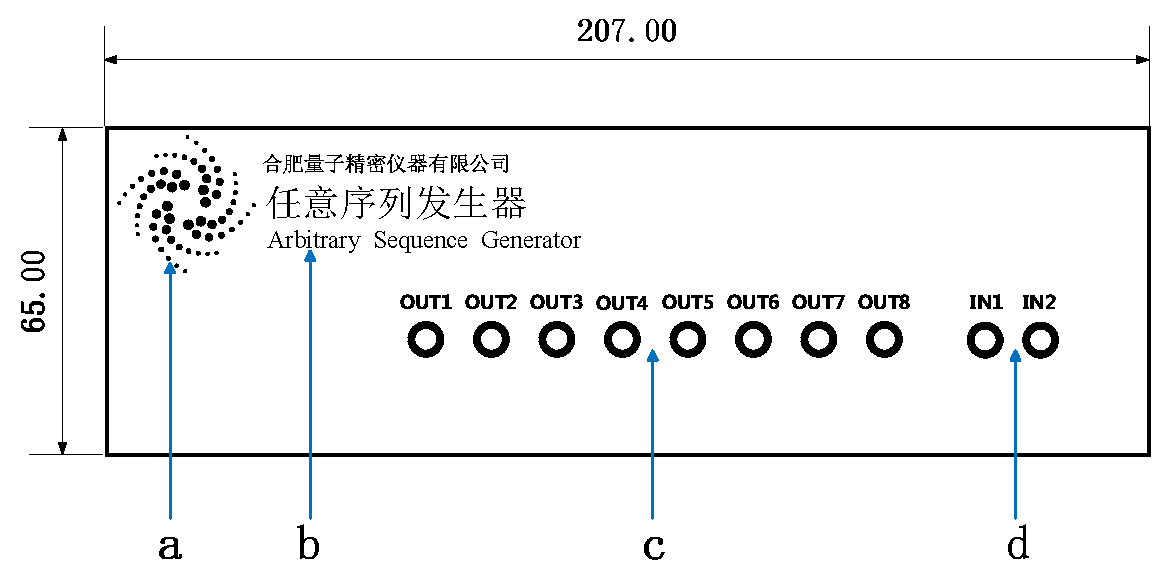
\includegraphics[width=14cm,height=6.5cm]{fig1_1}
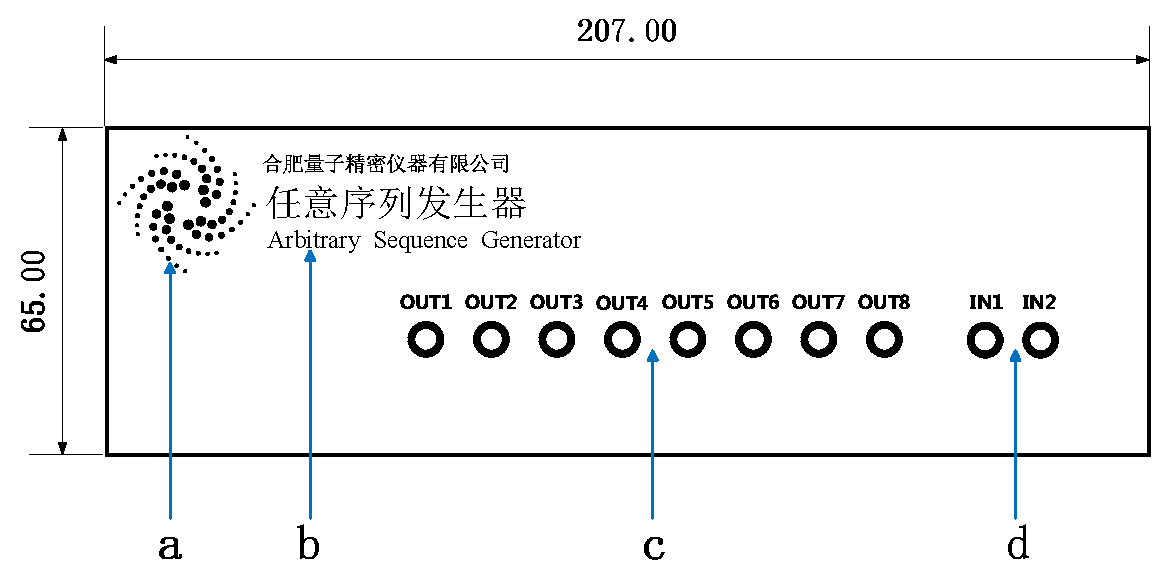
\includegraphics[height=6.5cm]{fig1_1}
\caption{机箱前面板}\label{fig:fig1_1}
\end{figure}

\noindent \textbf{a.} 合肥量子精密仪器有限公司注册商标。\\
\textbf{b.} 公司名称与产品名称。\\
\textbf{c.} 共 8 个方波输出通道。\\
\textbf{d.} 客户定制化功能通道。

%\newpage
\begin{figure}[ht]
\centering
%\includegraphics[width=14cm,height=6cm]{fig1_2}
\includegraphics[height=6cm]{fig1_2}
%\includegraphics[width=14cm,height=6cm]{houmianban}
\caption{机箱后面板}\label{fig:fig1_2}
\end{figure}
%\begin{enumerate}
%\item USB通信接口,通过USB连接线将仪器连接到计算机。
%\item “UART”为保留接口,用于客户定制化功能。共8个方波输出通道。
%\item 仪器开关按钮,“I”状态为开,“O”状态为关。
%\item 指示灯,仪器处于工作状态时亮起。
%\item 电源接口。
%\end{enumerate}

\noindent \textbf{e}. 通信接口,通过 USB 连接线将产品连接到计算机。\\
\textbf{f.} 客户定制化功能接口。\\
\textbf{g.} 开关按钮。\\
\textbf{h.} 指示灯,仪器工作时亮起。\\
\textbf{i.} 电源接口。

\begin{figure}[ht]
\centering
%\includegraphics[width=11.6cm,height=6.5cm]{fig1_3}
\includegraphics[height=6.5cm]{fig1_3}
\caption{机箱侧面板}\label{fig:fig1_3}
\end{figure}
%\begin{enumerate}
%\item 仪器通风口,用于仪器电路板散热。
%\end{enumerate}
\noindent \textbf{j.} 机箱通风口,用于仪器电路板散热。

\section{\heiti 连接电源}
ASG-GT50-C的供电电压为直流12 V。用户可使用直流稳压电源提供12 V直流电压,或使用随机箱附件提供的电源适配器将仪器连接至220 V,50 Hz的交流电源中。接通电源后,按下开关按钮,可以看到后面板的指示灯亮起,表示仪器已经处于工作状态。

